\chapter{Work Completed}

Time series line charts---of both the simple line chart and small multiples varieties---were chosen to display the biomass forecast data output by the model.  A major reason line charts were chosen is that casual viewers can understand them without further instructions, as opposed to, say a horizon graph.  Another advantage to line charts is that they tend to have a reasonable amount of whitespace where additional information can be displayed, such as uncertainty or alternate forecasts. A key design issue concerned the representation of change.  A number of alternatives were implemented and are described below.

Interaction with the model parameters is done by means of a set of sliders with the goal of allowing the user to immediately see the impact of management decisions.  The user can adjust sliders which represent harvest effort and watch the line charts change instantaneously as the model is re-run according to the new effort values.  Like Eberlein and Peterson, we aimed to turn the ``time consuming and tedious'' task of working with a model into a ``fast and fun'' interactive experience \cite{eberlein1992}.  Different views and features of the visualization are discussed in the sections below.  

%%%

\section{Visualization of Change}

In addition to the blended visualization of change mentioned in Section~\ref{sec:displayingChange}, we will introduce an alternative of the prior values represented simple curve without blending between the curves.

\section{Visualization of Inter-Species Relationships}

As described in Section~\ref{sec:betweenSpeciesArcs}, users can toggle between no interspecies arcs, predation arcs, and interaction arcs.  An alternative will be developed where arcs of both types appear only selectively---i.e., an arc representing the effect of ``Species A'' on ``Species B'' will only appear if some change in effort values resulted in the biomass of ``Species B'' changing.

\section{Visualization of Uncertainty}

The output of all scientific models is best understood as a range of expected values, since models are merely simplifications of reality.  Therefore, we will perform Monte Carlo simulations by randomly jittering the non-zero input parameter values $\pm 10\%$ for the MS-PROD model.  The resulting uncertainty will be displayed in one of the following methods:

 \begin{itemize}
   \item Multi-line (one semi-transparent line per Monte Carlo simulation run)
   \item Error bars of standard deviations
   \item Error bands of standard deviations
   \item Error boxes of quartiles
 \end{itemize}


%%%%

\section{Functional Group View}

\begin{figure}[h]
	\centering
	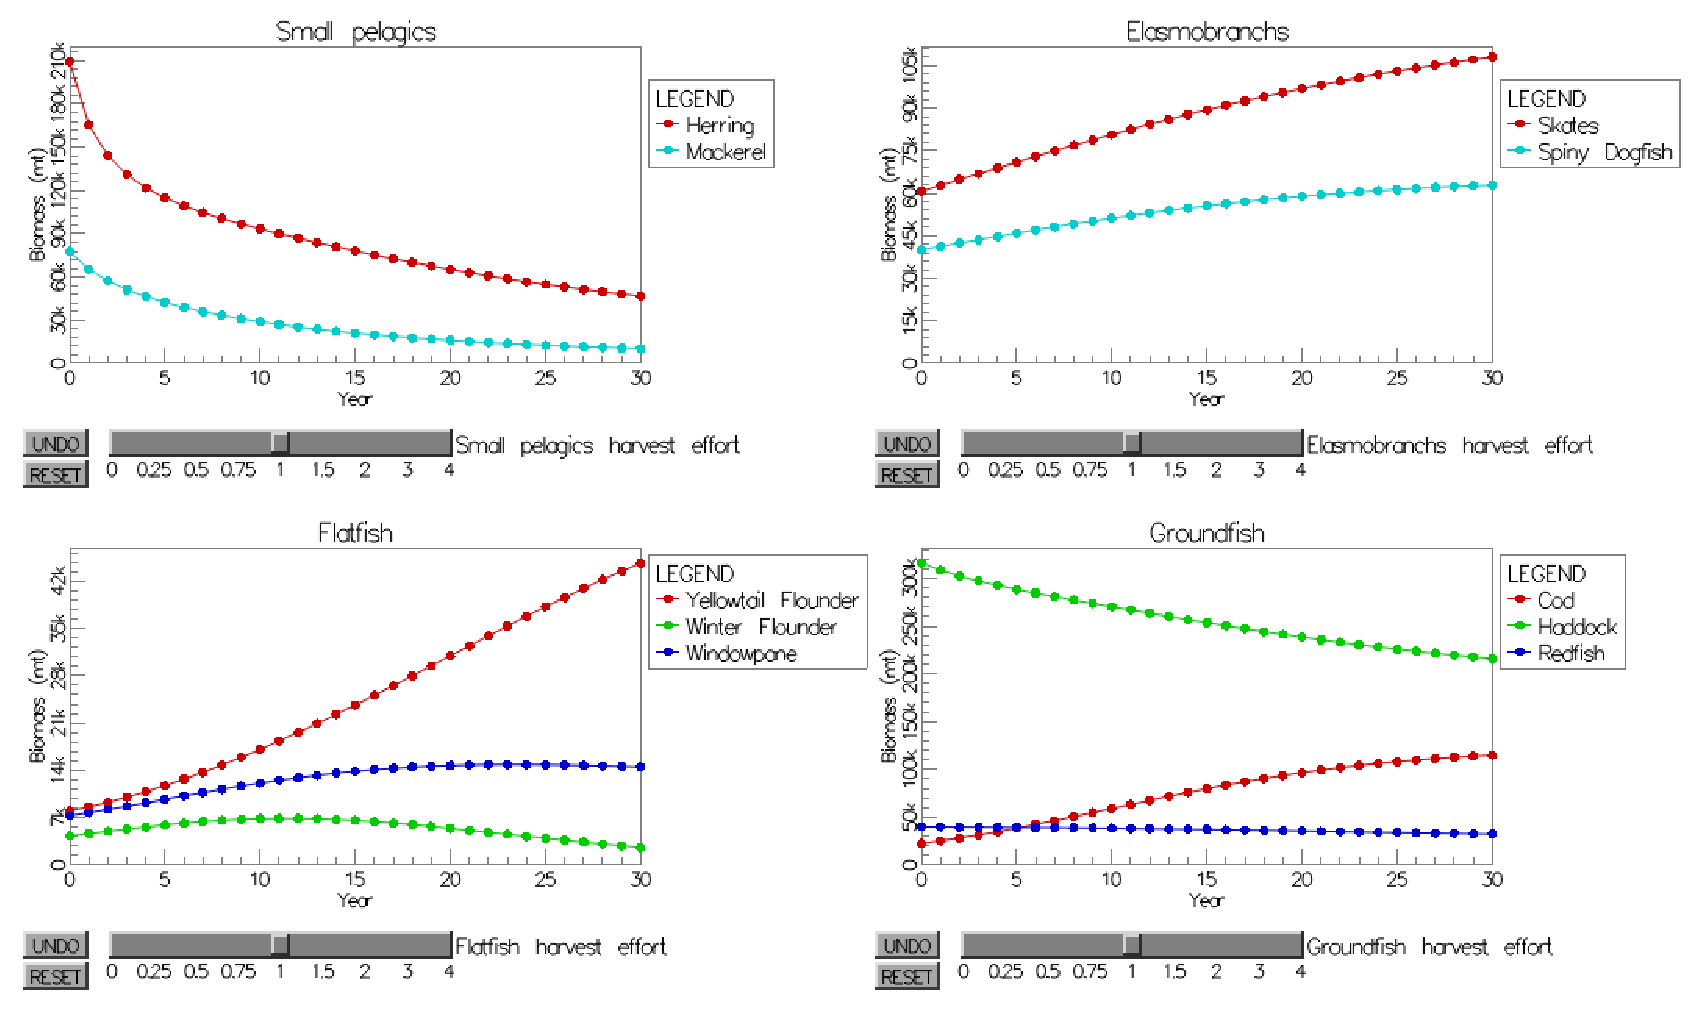
\includegraphics[width=15cm]{figures/eps/msprod_group.eps}
	\caption{A ``by group'' view of our MS-PROD visualization.}
	\label{fig:msprod_group}
\end{figure}

Early on in the design process, a design was made to organize the time series plots according to functional group.  A functional group is a biological grouping of species which perform similar functions within their ecosystem---e.g., mackerel and herring are both members of the ``small pelagic'' group since they live in the water column.  There were three reasons for this design decision.  First, it is difficult to select enough distinct colors to represent each species so that all species could be plotted on a single chart.  Second, the biomass of some species was significantly larger than others, which was also problematic when all species were on one chart.  By scaling the $y$-axis according to the largest biomass value in the entire 30-year timespan, the lines representing some species were crowded at the bottom of the chart and seemed to be flat even when they were not.  It was then observed that species of similar functional groups tend to have biomass values in similar numeric ranges.  Third, harvest effort is controlled by functional group, so it made sense to develop a line chart for each functional group.  Figure~\ref{fig:msprod_group} shows a screenshot of biomass predictions produced by the model and displayed by these four functional groups.

%The MS-PROD model requires that the functional group of each species is specified in the input parameter file; the four featured in the input file used for the majority of the development were small pelagics, elasmobranchs, flatfish, and groundfish.  

The major advantage of this ``by group'' view is that comparisons of species within a group are easy.  For MS-PROD, there are only two or three species per functional group, so the line chart for each group tends to not suffer from occlusion problems, unlike with the initial single line chart approach.  Direct and indirect effects of changes in harvest effort also become more clear with the ``by group'' approach---e.g., if the user adjusts the effort slider only for elasmobranchs, yet sees the biomasses change on the groundfish chart, then the user can begin to understand there is some kind of relationship between elasmobranchs and groundfish.

\section{Species View}

\begin{figure}[h]
	\centering
	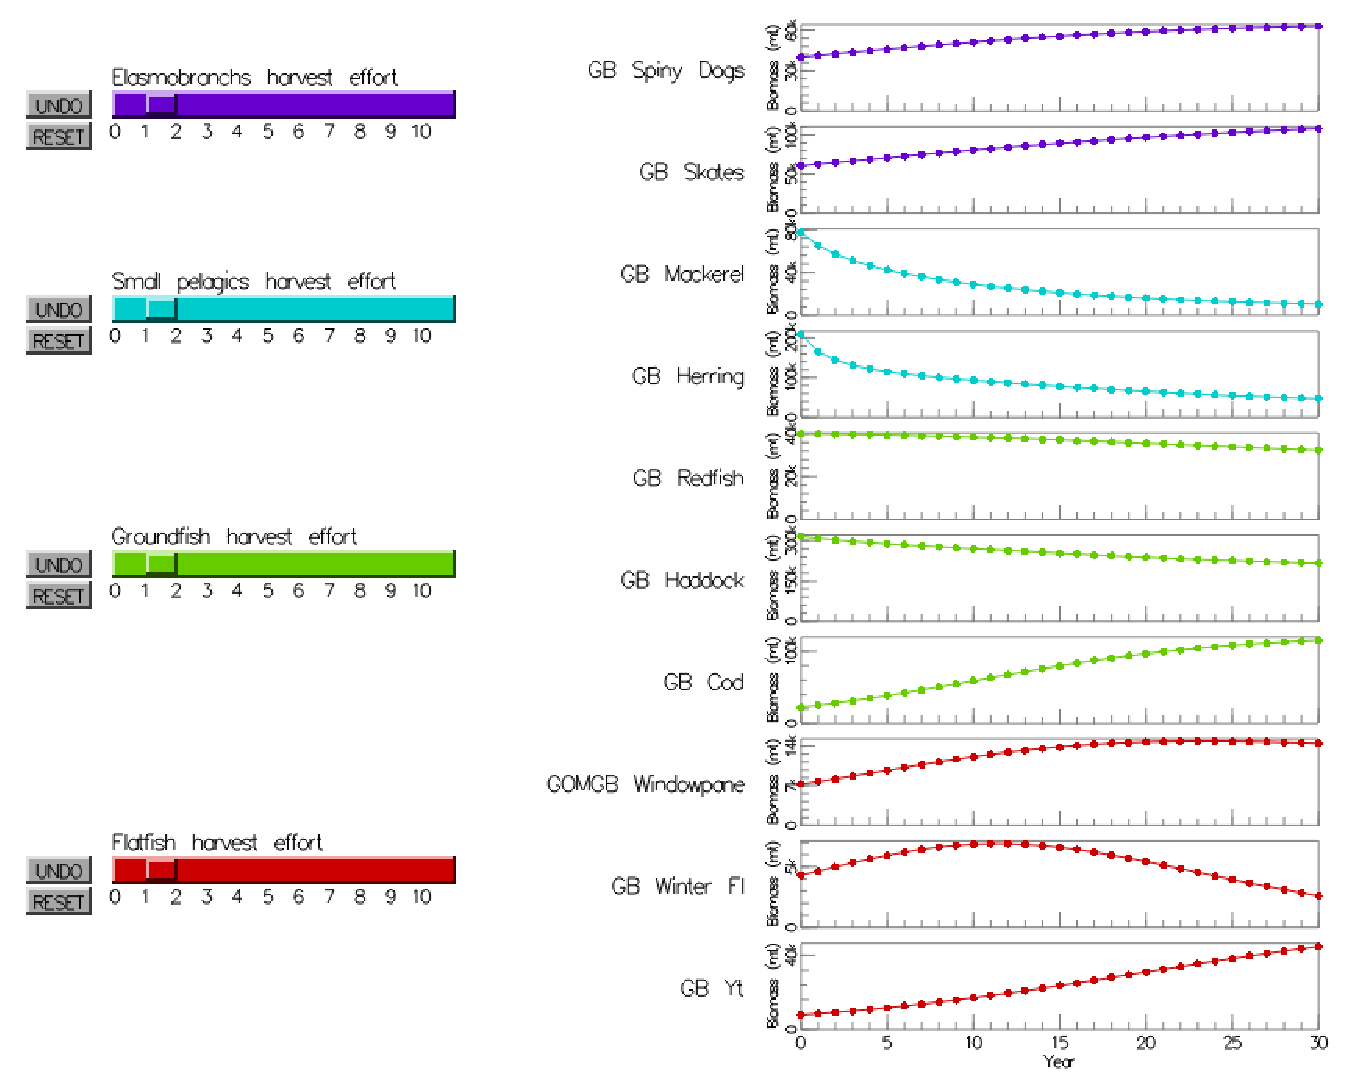
\includegraphics[width=13cm]{figures/eps/msprod_species.eps}
	\caption{A ``by species'' view of our MS-PROD visualization.}
	\label{fig:msprod_species}
\end{figure}

The alternative to viewing ``by group'' is to view each species on its own plot, as in small multiples.  In this style, each plot is sorted and colored according to functional group membership, as seen in Figure~\ref{fig:msprod_species}.  The harvest effort sliders are also colored by functional group and positioned near the plots of the corresponding group.  This allows for the ability to differentiate between direct and indirect effects of changes in harvest effort.

With each species on its own plot, it is much easier to interpet the biomass predictions of an individual species, since the $y$-dimension of a plot needs to be scaled to the data of one species only.  It is easier to perceive increases or decreases in biomass because no species suffers from the flattening that can occur when a series is displayed on the same plot as a series that has significantly higher values.  On the other hand, this makes comparison between species somewhat difficult because the user must either refer to the $y$-axis labels or hover over a specific point on a chart in order to determine the absolute value of the biomass at a point in time.

\subsection{Absolute Size Indicators}

\begin{figure}[h]
	\centering
	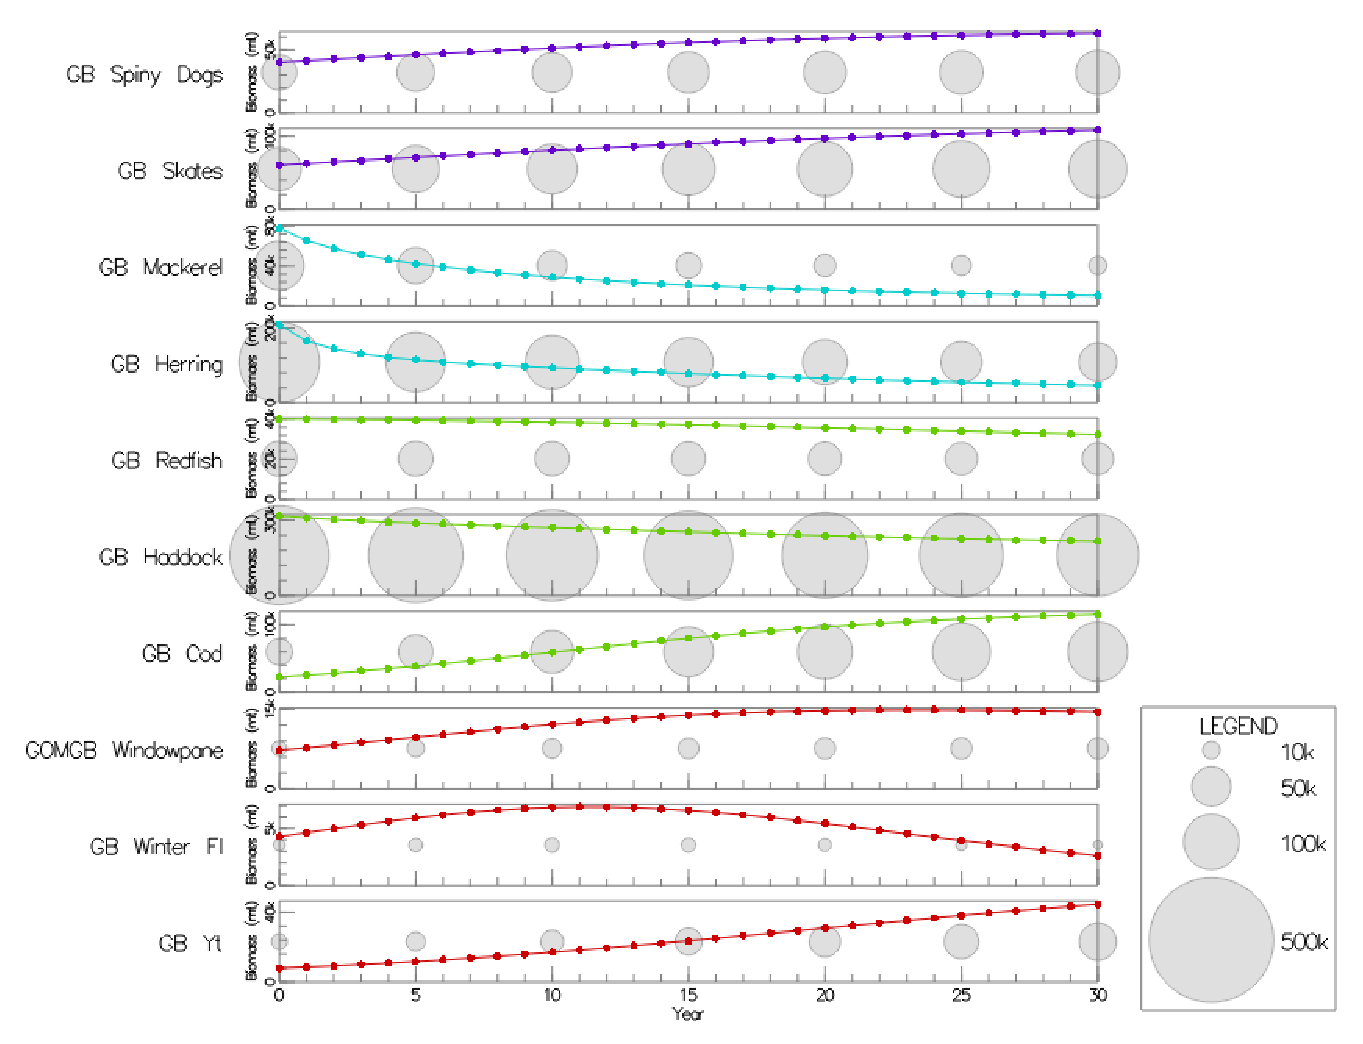
\includegraphics[width=12cm]{figures/eps/msprod_abssize.eps}
	\caption{Absolute size indicators overlaying the ``by species'' view.}
	\label{fig:msprod_abssize}
\end{figure}

In the ``by species'' view, the scaling of the $y$-dimension is adjusted to fit the data of each individual chart.  Therefore, as mentioned, it is difficult to ascertain the absolute biomass sizes in order to compare between species.  The introduction of absolute size indicators, seen in Figure~\ref{fig:msprod_abssize}, alleviates this problem by showing the absolute size of the population as the area of a circle.  To avoid occlusion, these indicators are drawn every five years within the thirty-year timespan, but they still make for quick comparison between different species.

\subsection{Between Species Arcs} 
\label{sec:betweenSpeciesArcs}

The predictions for biomass in this model take inter-species relationships into account.  These relationships are \textit{predation}, where one species consumes another, and \textit{interaction}, which accounts for the way any spcies might impact another that is not predation.  Understanding these relationships may be critical to understanding why some a species fish is indirectly affected by fishing efforts of other types of fish.  Therefore, we chose to include a network visualization of these relationships in our application, as seen in Figure~\ref{fig:betweenSpeciesArcs}.

\begin{figure}
\centering
	\begin{subfigure}[b]{0.48\textwidth}
		\centering
		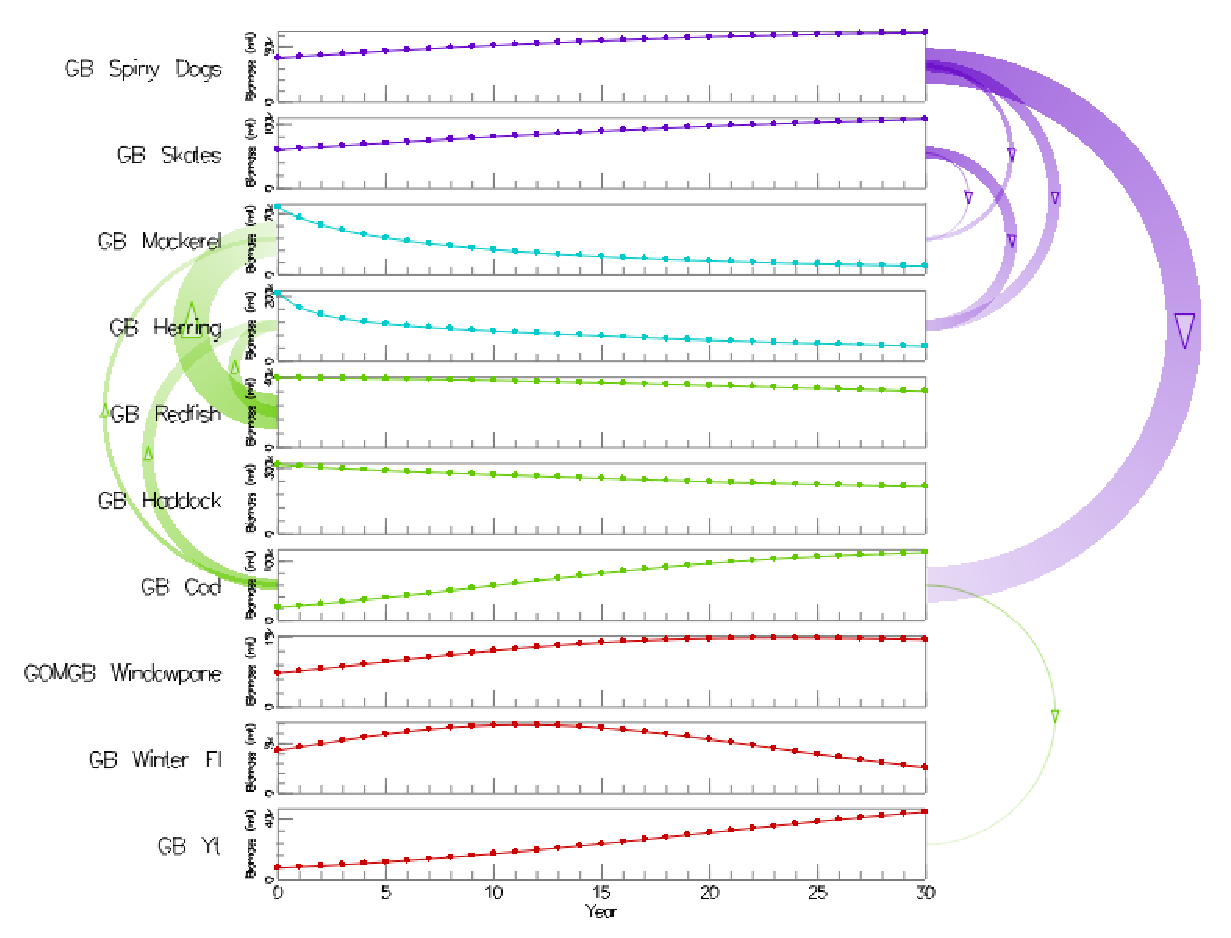
\includegraphics[height=4.5cm]{figures/eps/arcs_predation.eps}
		\caption{Predation arcs.}
		\label{fig:arcsPredation}
	\end{subfigure}	
	\begin{subfigure}[b]{0.48\textwidth}
		\centering
		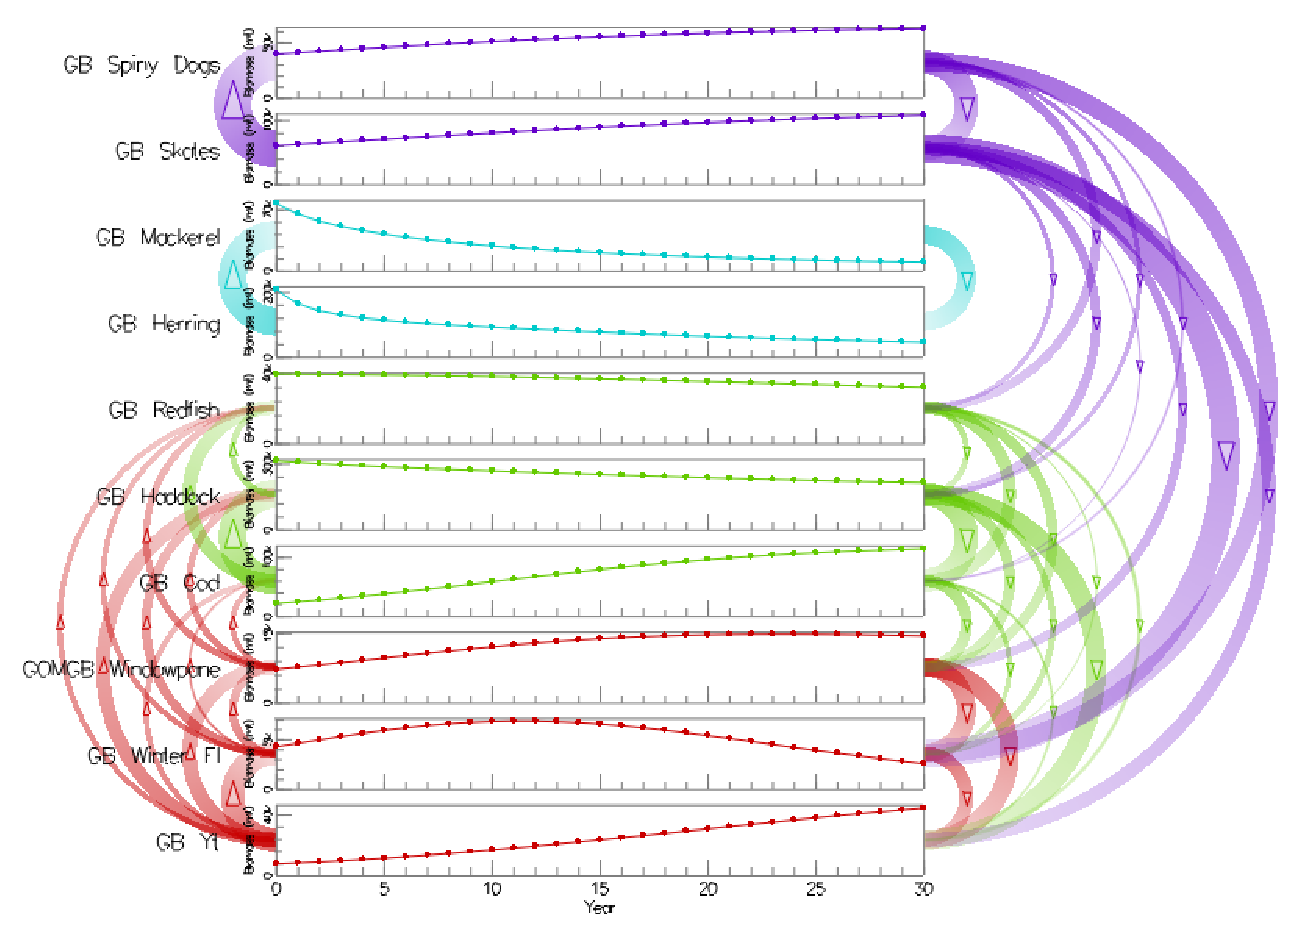
\includegraphics[height=4.5cm]{figures/eps/arcs_interaction.eps}
		\caption{Interaction arcs.}
		\label{fig:arcsInteraction}
	\end{subfigure}
	\caption{Arcs drawn between species charts to represent relationships.}
	\label{fig:betweenSpeciesArcs}
\end{figure}

The arc diagram was selected over other network visualizations because it is easily integrated into our time series visualizations.  A separate node-link diagram, such as one with a force-directed layout, may have been confusing because it would require the user to mentally associate nodes in the network with line charts.  As mentioned previously, Heer et al. described a major benefit of the arc diagram is that the one-dimensionality allows for other features to be easily displayed near the nodes \cite{heer2010}.  In our case, the time series line charts are the nodes; the line charts are only enhanced, not occluded, by the arcs.  Arc diagrams are also well suited to smaller datasets with clusters of nodes, which applies to our dataset since the fish are segmented into functional groups.

\section{Displaying Change}
\label{sec:displayingChange}

The motivation of this visualization is to allow the modelers and other stakeholders to easily run the MS-PROD model in order to compare the effects of different choices of fishing effort.  Thus, the visualization requires some method of comparing alternate biomass forecasts and granting users the ability to decide which fishing effort values seem most sustainable.  Therefore, we have added a feature which allows the user to save a ``base line'' of fishing effort values, change the fishing effort values, and compare the new biomass predictions to those of the original base line.

\begin{figure}[h]
	\centering
	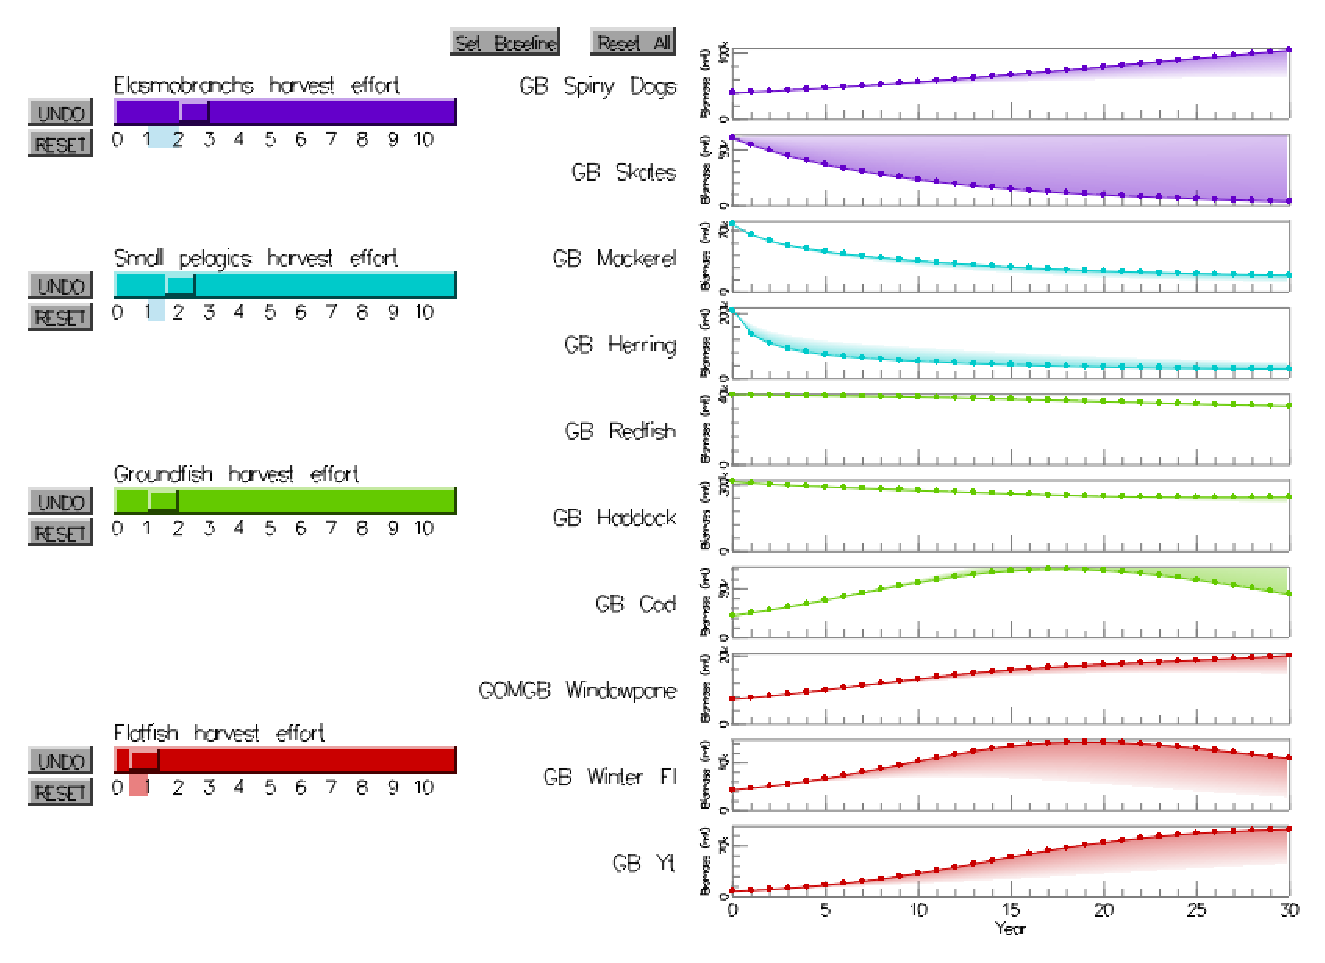
\includegraphics[width=12cm]{figures/eps/msprod_change.eps}
	\caption{Showing change between different effort values.}
	\label{fig:msprod_change}
\end{figure}

Figure~\ref{fig:msprod_change} shows this feature which displays change.  The blended area in a line chart is colored from the current biomass line to the line as it was when the baseline was set; a colored area above the line indicates the biomass declined, while a colored area beneath represents the biomass increased---e.g., the ``skate'' population declined dramatically with the new effort values, the ``winter flounder'' population increased due to the changes, and ``haddock'' seemed to be unaffected.

Underneath the sliders, the colors---if present---indicate how the baseline effort values were set.  Blue indicates the effort value has been increased since the baseline was set---e.g., again in Figure~\ref{fig:msprod_change}, the effort for ``elasmobranchs'' was originally set to 1.0 and now it is approximately 2.0.  Red represents the effort value has been decreased since the baseline was set---e.g., the effort for ``flatfish'' was originally set to 1.0 and now it is approximately 0.5.

This feature is available in both the ``by group'' and ``by species'' views.  The baseline can be saved at any time with a simple button at the top of the screen.  Buttons are also available to undo or reset changes to the effort values.
